% Poster

% Define the coument as a beamer
\documentclass{beamer}

%%%%%%%%%%%%%%%
%%% Import Pakages %%%
%%%%%%%%%%%%%%%

\usepackage{graphicx}  % Ability to import figures
\usepackage{amsmath} % This and next two will allow use of amthematical symbols, theorems, definitions, etc.
\usepackage{amsthm}
\usepackage{amssymb}
\usepackage{ragged2e} % Allows text allignment commands, including \justify
\usepackage{syntonly}  % Allows \syntax only to be used
\usepackage{array}        % Allows table modifications
\usepackage{colortbl}    % Allows the coloring of tables
\usepackage{tcolorbox} % Allows colorable outlines, among other features
\usepackage{caption}
\usepackage{lipsum} % Allows use of lorem lipsum
\usepackage[export]{adjustbox}
\usepackage{soul}
\usepackage{tikz}
\usepackage{transparent}
\usepackage[orientation = landscape, size = a0, scale = 1.4]{beamerposter}  % Turns beamer into a poster
% Scaling is font scaling

% Set the frame margins to make sure everything fits more 'snuggly' into the frame
\setbeamersize{text margin left = 2em, text margin right = 2em}

% Set up  title information
\title{Short-term Monitoring and Forecasting of Flash Drought Conditions}
\author{Edris, S., J. Basara, J. Christian, R. Wakefield}
\date{}

% Define some colors
\definecolor{OUcrimsion}{RGB}{130,50,50}
\definecolor{OUcream}{cmyk}{0.02,0.03,0.09,0}

%%%% Some Colorboxes may need to be made for this. See the Example_Poster.tex for more on this %%%%
\tcbuselibrary{skins} % Allows use of other skins
\newtcolorbox{creambox}{skin = enhanced, arc = 5mm, colback = OUcream, %colframe = OUcream, opacityframe = 0.5
                                               frame style = {inner color = OUcream, outer color = OUcrimsion}}

% Make the normal blocks transparent, and allow tcolorboxes to handle the background.
\setbeamercolor{block title}{fg = black, bg = }
\setbeamercolor{block body}{fg = black, bg = }

% Set some beamer features
\setbeamercolor{background canvas}{bg = OUcrimsion}
\setbeamercolor{itemize item}{fg = black}
\setbeamercolor{itemize subitem}{fg = black}
\setbeamercolor{enumerate item}{fg = black, bg = }
\setbeamercolor{enumerate subitem}{fg = black, bg = }
\setbeamercolor{bibliography item}{fg = black, bg = }

\setbeamertemplate{items}[circle]
\setbeamertemplate{enumerate items}[default]
\setbeamertemplate{bibliography item}[triangle]

%\syntaxonly % Use to increase compliation speed and test for errors, but suppress output.


%%%%%%%%%%%%%%%%
%%% Begin the Poster %%%
%%%%%%%%%%%%%%%%

\begin{document}
	\begin{frame}[t]{}
		%%%%%%%%%%%%%%%%%%
		%%% Set the Title Section %%%
		%%%%%%%%%%%%%%%%%%
		
		\section{title} % Adds a shortcut in TeXStudio
		
		% Section is divided into three column
		% Left column is a logo(s)
		% Middle is the title, authors, and affiliation
		% Right column is logo(s)
		
		\begin{columns}
			\column{0.13\textwidth}
			~~~~~~ % Creates white spaces to center the logo(s)
%			
\includegraphics[width = 0.40\textwidth]{../Figures/Poster/SoMLogo.png}
%			~~
			\begin{figure}[htp]
				
\includegraphics[width = 0.43\textwidth]{../Figures/Poster/ou_logo.png}
			\end{figure}
			
			%This logo is a placeholder
			
			\column{0.65\textwidth}
			~~~~~~ % Creates white space to center the title
			\begin{creambox}
				\begin{block}{} % Could turn into a predefined block for the title
					\centering
					\bf\textsc{\LARGE Short-term Monitoring and Forecasting of Flash Drought Conditions}\vspace{0.25em}
					\par
					\textsc{Stuart G. Edris$^{1,3}$, Jeffrey B. Basara$^{1,2}$, Jordan I. Christian$^1$, Ryann A. Wakefield$^1$}\vspace{0.25em}
					\par
					\textsc{${}^1$School of Meteorology, University of Oklahoma, Norman, Oklahoma \\ ${}^2$School of Civil Engineering and Environmental Science, University of Oklahoma, Norman, Oklahoma}\vspace{0.25em}
					\par
					\textsc{$^3$Contact: sgedris@ou.edu} % Fill in the contact information
				\end{block}	
			\end{creambox}
			
				
				\column{0.20\textwidth}
				~~ % White spaces to center the logo(s)
				
\includegraphics[width = 0.398\textwidth]{../Figures/Poster/SoMLogo.png}
				\hspace*{-0.3cm}
				
\includegraphics[width = 0.40\textwidth]{../Figures/Poster/HWS-Logo.png}
				%This is still a placeholder logo
		\end{columns}
		\vspace*{0.0cm} % Removes some blank space between title/logos and proceding columns
		
		% Remainder of poster is contained within two overarching columns
		\begin{columns}[t]
			\column{0.40\textwidth}
			
			%%%%%%%%%%%%%%%%%%%%%%%%%%
			%%% Introduction/Bakcground Sections %%%
			%%%%%%%%%%%%%%%%%%%%%%%%%%
			
			\section{Introduction} % Adds a shortcut within TeXStudio
			
			\begin{creambox}
				\begin{block}{\bfseries Introduction}
					\justify
					Flash droughts are droughts that develop over rapid time scales ($\thicksim 1$ month) and have high impact on vegetation and agriculture. % Needs much better wording here.
					As such, being able to properly identify and predict flash droughts is important, though there has been some debate on how to identify and classify flash droughts (Otkin et al. 2018). %~\citep{Otkin_2018}.
					A method to identify and quantify flash drought has recently been developed by Christian et al. (2019). %~\cite{Christian_2019}.
					This method was developed for the NARR, so it can only identify flash droughts retrospectively, though it should work for any gridded system. 
					Hence, this study takes the method developed in Christian et al. (2019)~%~\cite{Christian_2019}
					and attempts to apply it to the GFS to identify flash droughts in real time and obtain short-term forecasts. Early focus has been given
					to the flash drought in 2012 to develop and test the algorithm for the GFS as 2012 drought conditions are known (e.g., Christian et al. 2019 and  Basara et al. 2019).
				\end{block}
			\end{creambox}
			
			%%%%%%%%%%%%%%%%%%%%%
			%%% Data and Methods Section %%%
			%%%%%%%%%%%%%%%%%%%%%
			
			\section{DataMethods} % Adds a shortcut to TeXStudio
			
			\begin{creambox}
				\begin{block}{\bfseries Data and Methods}
					\begin{columns}[t]
						%\justify
						\column{0.48\textwidth}
						Data was collected from:
						\begin{itemize}
							\item GFS $1^{\circ} \times 1^{\circ}$ data. Temporal resolution of 3 hours out to 192 hours (8 days).
							\begin{itemize}
								\item A minimum of 30 day dataset of 3 hour forecasts was constructed and combined with a full model run
								\item The 0 hour forecast is the beginning of the full model run
							\end{itemize}
							\item NARR $32\text{km} \times 32\text{km}$ data. Daily mean ESR values provided from Jan. 1 1979 to Dec. 31 2016.
						\end{itemize}
						Data extracted from the GFS included:
						\begin{itemize}
							\item Surface latent heat flux (LE)
							\item Potential evaporation rate (PET)
						\end{itemize}
						The following variables were calculated obatined from both datasets:
						\begin{itemize}
							%\item Evaporative stress ratio ($\text{ESR} = \frac{\text{LE}}{\text{PET}}$; daily average)
							\item Standardized evaporative stress ratio ($\text{SESR} = \frac{\text{ESR} - \overline{\text{ESR}}}{\sigma _{\text{ESR}}}; \quad \text{ESR} = \frac{\text{LE}}{\text{PET}}$)
							\begin{itemize}
								\item Daily averaged SESR was used for criteria 2
								\item Pentad (5 day average) SESR was used to calculate $\Delta \text{SESR}$ for criteria 3 and 4 as they better represent the trend
							\end{itemize}
							\item $\Delta \text{SESR} = \text{SESR}_{t} - \text{SESR}_{t-1}$
							\item $\Delta \text{SESR}$ was also standardized
							\item Means and standard deviations were obtained from the daily NARR dataset
						\end{itemize}
					
						\begin{figure}
							\captionsetup{width = 0.95\textwidth}
							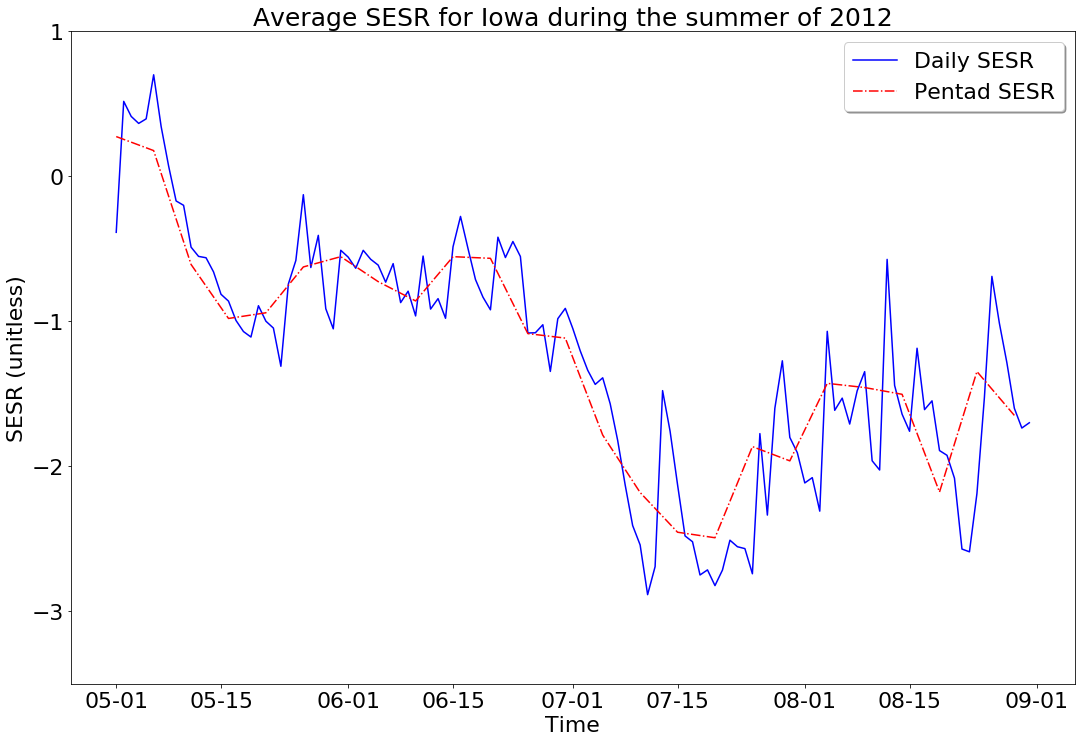
\includegraphics[width = 0.95\textwidth, frame]{../Figures/Poster/Daily_SESR_vs_Pentad_SESR.png}
							\caption{Daily and Pentad SESR for Iowa during the summer of 2012, calculated from the NARR.}
						\end{figure}
						
						\column{0.48\textwidth}
						Flash drought was identified using the same 4 criteria in Christian et al. (2019)%~\cite{Christian_2019}
						\begin{enumerate}
							\item There must be a minimum of 30 days between start and end dates
							\item The final SESR value must be below the 20th percentile
							\item The following must be true:
							\begin{enumerate}[a)]
								\item $\Delta \text{SESR}$ for each date in the flash drought must be below the 40th percentile
								\item No more than 1 exception is allowed for criteria 3a
							\end{enumerate}
							\item The mean $\Delta \text{SESR}$ between start and end dates must be below the 25th percentile
						\end{enumerate}
						For purposes of identification and forecasts, every day in the GFS forecast were treated as end dates.
						
						\begin{figure}
							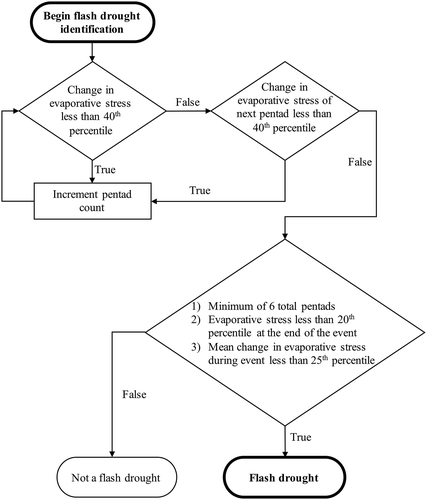
\includegraphics[height = 10in, frame]{../Figures/Poster/Christian_2019_Fig3.png}
							\caption{\normalsize Algorithm used to identify flash drought using SESR and $\Delta \text{SESR}$. Figure 3 in Christian et al. (2019).}%~\cite{Christian_2019}
						\end{figure}
					\end{columns}
				\end{block}
			\end{creambox}
			
		
			% Move to the second overarching column
			\column{0.60\textwidth}
			
			%%%%%%%%%%%%%%%%%%%%%%
			%%% Priliminary Results Section %%%
			%%%%%%%%%%%%%%%%%%%%%%
			
			\section{PreliminaryResults} % Adds a shortcut to TeXStudio
			
			\begin{creambox}
				\begin{block}{\bfseries Priliminary Results}
					\vspace*{-1.5cm} % Removes some blank space between title and columns
					\begin{columns}[t]
						\column{0.60\textwidth}
						\begin{figure}[htp]
							\captionsetup{width = 0.95\textwidth}
							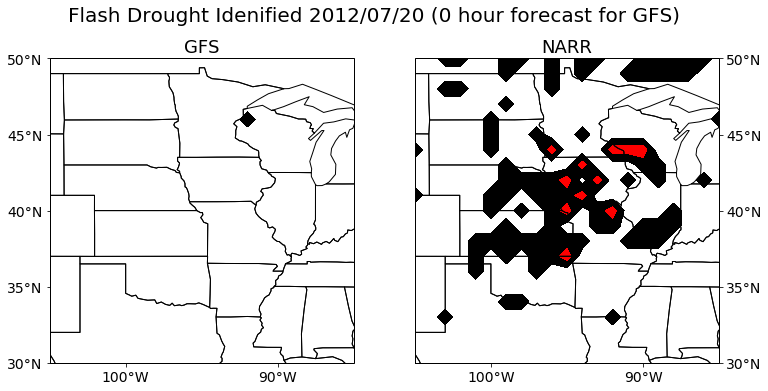
\includegraphics[width = 0.95\textwidth, frame]{../Figures/Poster/Flash_Drought_Identified_20120720.png}
							\caption{\normalsize Flash drought identified by GFS (left) and NARR (right) for the Great Plains on July 20, 2012. Red indicates what the GFS would have identified with 1 month of data.}
						\end{figure}
					
						\column{0.40\textwidth}
						\begin{figure}[htp]
							\captionsetup{width = 0.95\textwidth}
							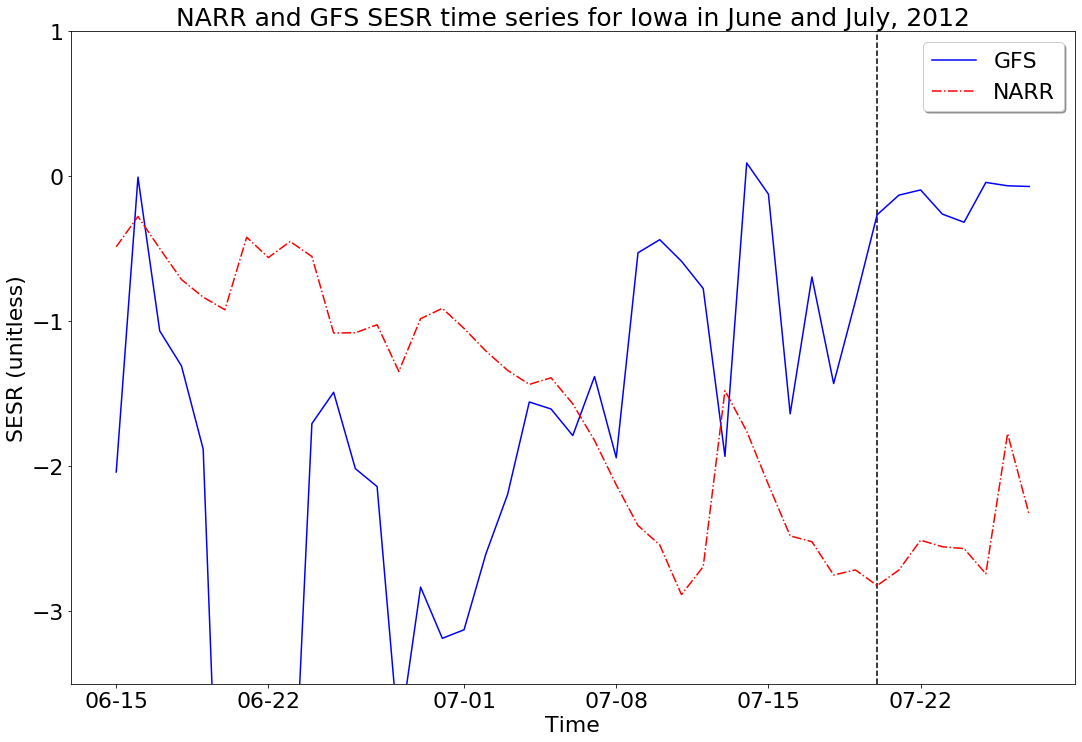
\includegraphics[width = 0.95\textwidth, frame]{../Figures/Poster/SESR_timeseries_for_NARR_GFS.png}
							\caption{\normalsize SESR time series in Iowa during the 2012 flash drought for the GFS (solid blue line) and NARR (dashed red line). The black dashed line indicates the 0 hour forecast.}
						\end{figure}
					\end{columns}
					
					\vspace*{-0.25cm} % Removes some blank space between figures
					\begin{columns}[t]
						\column{0.65\textwidth}
						\begin{figure}[htp]
							\captionsetup{width = 0.95\textwidth}
							{\setlength{\fboxsep}{0pt}%
								\fbox{%
								\begin{minipage}{0.95\textwidth}
									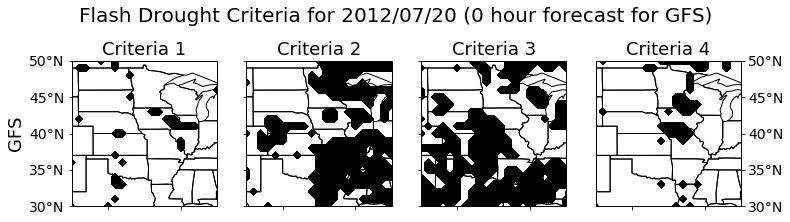
\includegraphics[width = 1.0\textwidth]{../Figures/Poster/GFS_criteria_20120720.png}
									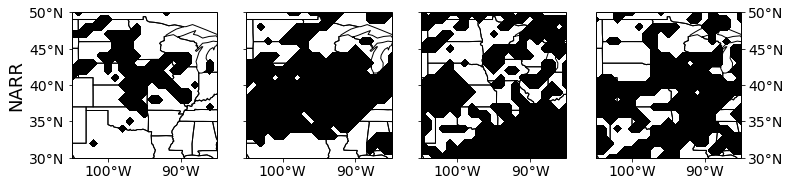
\includegraphics[width = 1.0\textwidth]{../Figures/Poster/NARR_criteria_20120720.png}
								\end{minipage}}} % fbox is an alternate to add a frame
							\caption{\normalsize Each flash drought criteria for the GFS (top) and NARR (bottom) for the Great Plains in July 20, 2012.}
						\end{figure}
					
						
						\column{0.35\textwidth}
						\begin{itemize}
							\item GFS seems to have trouble reproducing SESR and associated trends
							\begin{itemize}
								\item It is currently unknown if this may be due to calculation errors or errors in the GFS
							\end{itemize}
							\item This results in the GFS not having a rapid enough drying period
							\begin{itemize}
								\item Criteria 3 fails quickly, resulting in a small area where criteria 1 is true
								\item The overall trend is also heavily underestimated, resulting in a failed criteria 4
							\end{itemize}
							\item As an interesting note, the GFS will not see the entire drought
							\begin{itemize}
								\item The GFS only identify flash drought that began at the start of its 30 day dataset. If the drought began before that dataset, the GFS will not identify it.
								\item E.g., the figures identifying flash also show flash drought identified at earlier times. For the NARR, this includes May and June  (before the GFS dataset starts). What the GFS would have seen with its 1 month dataset is indicated in red.
							\end{itemize}
						\end{itemize}
					\end{columns}
					
				\end{block}
			\end{creambox}
			
			%%%%%%%%%%%%%%%%%%
			%%% Conclusions Section %%%
			%%%%%%%%%%%%%%%%%%
			
			\section{Conclusions} % Adds a shortcut to TeXStudio
			
			\begin{creambox}
					\begin{columns}[t]
						\column{0.50\textwidth}
						\vspace*{-0.5cm} % Removes some blank space between items and title
						\begin{block}{\bfseries Future Work}
							\begin{itemize}
								\item There is notable difference in SESR between the GFS and NARR models. 
								\item Currently, the forecast only goes until the GFS resolution changes. This is being worked on to obtain a flash drought forecast for the entire GFS run.
								\item The efficiency of the current algorithm needs to be improved.
								\item Flash drought that develops before or during the GFS dataset needs to be addressed.
								\item Once refined, the algorithm will be applied to other flash drought events to quantify the GFS's skill in identifying and forecasting flash drought.
							\end{itemize}
						\end{block}
					
						\column{0.28\textwidth}
						\vspace*{-1.0cm}
						\begin{block}{\bfseries\small Acknowledgements}
							\vspace*{-0.5cm}
							\justify
							This work was supported, in part, by the NOAA Climate Program Office's Sectoral Applications Research Program (SARP) Grant NA130AR4310122,
							the Agriculture and Food Research Initative Competitive Grant no. 2012-02355, from the USDA National Institute of Food and Agriculture,
							the USDA National Institute of Food and Agriculture (NIFA) Grant no 2016-6800224967, 
							the NASA Water Resources Program Grant 80NSSC19K1266, 
							and the USDA Southern Great Plains Climate Hub.
						\end{block}
						
						\column{0.20\textwidth}
						\vspace*{-1.0cm} % Removes some blank space between items and title
						\begin{block}{\bfseries\small References}
							{\tiny
							  \setbeamercolor{bibliography entry author}{fg = black}
							  \bibliographystyle{ametsoc2014}
							  \bibliography{../Article_Notes/Thesis_bibliography}
						   	  \nocite{Otkin_2018, Christian_2019, Basara_2019}}
						\end{block}
					\end{columns}
			\end{creambox}
		
		\end{columns}	
		
	\end{frame}
\end{document}



